\section{Δημοσίευση πακέτου \texttt{HierarchicalTemporalMemory.jl}}

	Στο πλαίσιο αυτής της εργασίας, ακολουθώντας την υλοποίηση του κεφαλαίου \ref{impl} και επαυξάνοντας πάνω σε αυτήν,
	δημιουργήθηκε πακέτο Julia που υλοποιεί τους 2 αλγορίθμους HTM που περιγράφηκαν.
	Δημοσιεύεται ως ελεύθερο λογισμικό \parencite{stallmanFreeSoftwareFree2002} στο Github\footnote{Ημερομηνία δημοσίευσης: 2019/06/09}:
	\url{https://github.com/Oblynx/HierarchicalTemporalMemory.jl}

	Η ανάπτυξη θα συνεχιστεί πέρα από το πλαίσιο αυτής της εργασίας.

\subsection{Συνεισφορές στο οικοσύστημα της Julia («upstream»)}

	\subsubsection{Διόρθωση στον πολλαπλασιασμό αραιού πίνακα με διάνυσμα}

	Η υλοποίηση της χρονικής μνήμης βασίστηκε στους αραιούς πίνακες.
	Η υποστήριξη των αραιών πινάκων στη Julia, αν και επαρκής για βασική χρήση, αφήνει μερικά κενά.
	Ένα τέτοιο διαπιστώθηκε κατά την εκπόνηση αυτής της εργασίας.

	Έστω αραιός πίνακας με τιμές Bool, \texttt{S::SparseMatrixCSC{Bool}},
	και πυκνό διάνυσμα Bool, \texttt{a::Vector{Bool}}.
	Ενώ εν γένει ο πολλαπλασιασμός αραιού πίνακα με πυκνό διάνυσμα υποστηρίζεται, αυτός ο συγκεκριμένος συνδυασμός τύπων δημιουργούσε πρόβλημα.
	Ο πολλαπλασιασμός κατά προεπιλογή πραγματοποιείται στον ημιδακτύλιο (+,*).
	Οι τελεστές αυτοί δεν έχουν ειδικό νόημα για τιμές Bool: \texttt{Bool + Bool} προκαλεί μετατροπή των ορισμάτων σε \texttt{Int} και εκτελεί εν τέλει \texttt{Int(Bool) + Int(Bool)}
	\footnote{ Δεν είναι δύσκολο να οριστεί ο πολλαπλασιασμός του αραιού πίνακα με το διάνυσμα σε διαφορετικό ημιδακτύλιο, πχ (max,min) --
	για την ακρίβεια αυτό ακριβώς παρουσιάζεται στο \cite{shahNovelAlgebrasAdvanced2013}, όπου δείχνεται ότι, για αραιούς πίνακες,
	η υλοποίηση από το χρήστη είναι πέρα από εύκολη και \textbf{εξίσου αποδοτική με τον τυπικό πολλαπλασιασμό που ορίζουν οι βασικές βιβλιοθήκες της γλώσσας} }.
	Επειδή και ο πίνακας και το διάνυσμα που συμμετέχουν στον πολλαπλασιασμό έχουν τύπο στοιχείου Bool,
	η συνάρτηση του πολλαπλασιασμού εσφαλμένα απέδιδε στο αποτέλεσμα τύπο στοιχείου Bool.
	Το επακόλουθο ήταν ο πολλαπλασιασμός $S*a$ να προκαλεί σφάλμα.
	Η προφανής επίλυση είναι η αλλαγή του τύπου του αποτελέσματος σε αυτό που προκύπτει από τις πράξεις μεταξύ των στοιχείων των ορισμάτων, εδώ \texttt{Int}.

	Καθώς η Julia αναπτύσσεται ως ελεύθερο λογισμικό, κατέστη εφικτό στο πλαίσιο αυτής της εργασίας να διορθωθεί αυτό το σφάλμα στην πηγή του.
	Η διόρθωση υποβλήθηκε ως «pull request» \footnote{\url{https://github.com/JuliaLang/julia/pull/32082}} και έγινε δεκτή.

	\subsubsection{Διόρθωση στο χειρισμό Unicode στο \texttt{Weave.jl}}

	Το κεφάλαιο \ref{impl} αυτής της αναφοράς συγγράφηκε με τη μεθοδολογία \textbf{«literate programming»} \parencite{knuthLiterateProgramming1984},
	που εμπλέκει λειτουργικό κώδικα και αφηγηματικό κείμενο,
	χρησιμοποιώντας το πακέτο της Julia \texttt{Weave.jl} \cite{pastellWeaveJlScientific2017}.
	Έγινε εκτενής χρήση χαρακτήρων Unicode που υποστηρίζονται από τη Julia, τόσο στο κείμενο όσο και στον κώδικα.
	Οι χαρακτήρες Unicode κωδικοποιούνται υπό το πρότυπο UTF-8, μια κωδικοποίηση μεταβλητού μήκους.

	Κατά τη δημιουργία της αναφοράς παρατηρήθηκε πρόβλημα στον τρόπο με τον οποίο το Weave.jl ερμήνευε τους χαρακτήρες Unicode.
	Από εκφράσεις με πολύ ειδικούς χαρακτήρες έλειπε το τελευταίο τμήμα.
	Διαπιστώθηκε λοιπόν ότι κατά την ανάγνωση του κειμένου το \texttt{Weave.jl} δε λάμβανε υπόψιν το μεταβλητό μήκος των χαρακτήρων UTF-8,
	θεωρώντας εσφαλμένα ότι κάθε χαρακτήρας έχει το ίδιο μήκος.
	Καθώς και αυτό είναι ανοιχτό λογισμικό, το σφάλμα επίσης διορθώθηκε στην πηγή του
	\footnote{\url{https://github.com/mpastell/Weave.jl/pull/215}}.
	Κατά τη συγγραφή αυτής της αναφοράς η αποδοχή της διόρθωσης εκκρεμεί.

\subsection{Παράδειγμα πρόβλεψης ακολουθίας} \label{conc:intro-tspred}

	Το πακέτο συμπεριλαμβάνει μία απλή εφαρμογή πρόβλεψης ακολουθίας, που χρησιμοποιήθηκε ως βασικός έλεγχος ορθότητας της υλοποίησης.
	Επομένως περιέχει τα υπόλοιπα στοιχεία που χρειάζεται ένα σύστημα πρόβλεψης με HTM και φαίνονται στο σχήμα (\ref{fig:sp}, πάνω):
	έναν κωδικοποιητή κι έναν αποκωδικοποιητή/κατηγοριοποιητή.

	\subsubsection{Κωδικοποιητής «απλός αριθμητικός»}

	Ο κωδικοποιητής αναπαριστά πραγματικούς αριθμούς φραγμένους σε ένα εύρος, δημιουργώντας SDR με μήκος N και πληθάριθμο w.
	Ο ελάχιστος αριθμός του εύρους αναπαρίσταται με το SDR που έχει τα w πρώτα bits ενεργά, αντίστοιχα ο μέγιστος έχει τα w τελευταία ενεργά.
	Κάθε ενδιάμεσος αριθμός αντιστοιχίζεται σε ένα ισοκατανεμημένο φάσμα μεταξύ των δύο ακραίων αναπαραστάσεων,
	ορίζοντας ουσιαστικά ένα σύνολο κλάσεων που διακριτοποιούν την είσοδο.
	Ο κωδικοποιητής αυτός ονομάζετα «απλός αριθμητικός».

	Η \textit{συγκόλληση k SDR στη σειρά} για μικρό k (πχ 2-7) είναι επαρκής τρόπος για τη συνδυασμένη αναπαράσταση k εισόδων.
	Οι διακριτές είσοδοι που συνδυάζονται με αυτήν την απλή λογική δεν μπορούν να είναι οσοδήποτε πολλές,
	γιατί η διάσταση του χώρου της εισόδου θα αυξηθεί πολύ πιο γρήγορα από την αύξηση της πληροφορίας που φέρει,
	δυσχεραίνοντας την αναγνώριση παρόμοιων εισόδων.
	Στο συνδυασμό πολλών εισόδων το κλειδί ενδέχεται να είναι η ιεραρχική οργάνωση πολλών μονάδων HTM,
	που θα αναλυθεί στις προτάσεις για μελέτη \ref{conc:study-suggestions}.

	\subsubsection{Αποκωδικοποιητής «SDR classifier»}

	Ο αποκωδικοποιητής, που ονομάζεται «SDR classifier» \parencite{cuiContinuousOnlineSequence2016},
	βασίζεται στην παρατήρηση ότι η δραστηριότητα της χρονικής μνήμης είναι η απεικόνιση ενός συμβόλου-εισόδου στο πλαίσιο των χρονικών του συμφραζομένων.
	Ο αποκωδικοποιητής που χρησιμοποιείται εδώ είναι ένα απλό ενός επιπέδου perceptron πολλών κλάσεων που μαθαίνει να συσχετίζει
	τη δραστηριότητα της χρονικής μνήμης με τις εισόδους του κωδικοποιητή.
	Η είσοδος είναι το διάνυσμα $Π$ των προβλέψεων της χρονικής μνήμης κι η έξοδος, κατανομή πιθανότητας πάνω στις κλάσεις του κωδικοποιητή.

	Έστω ο αποκωδικοποιητής $D$ καλείται να αποκωδικοποιήσει την πρόβλεψη $Π_t$, επιστρέφοντας
	$D(Π_t)$.
	Έστω επίσης ότι η πρόβλεψη αφορά την τιμή της εισόδου $k$ χρονικές στιγμές στο μέλλον,
	$u_{t+k}$.
	Τη στιγμή $t+k$, ο αποκωδικοποιητής θα χρησιμοποιήσει το σφάλμα $e_{t+k} = D(Π_t) - u_{t+k}$
	για να τροποποιήσει τον πίνακα βαρών $W$ του δικτύου του κατά
	$$ ΔW= -α .* e_{t+k}*Π[Π]' $$

	Για την ερμηνεία της κατανομής πιθανότητας στις κλάσεις του κωδικοποιητή απαιτείται και ένας μηχανισμός αποσαφήνισης.
	Παρέχονται 3 τέτοιοι: πιθανότερο ενδεχόμενο, μέσος όρος, μέσος όρος των πιθανότερων ενδεχομένων.


\section{Επαλήθευση βασικών ιδιοτήτων των αλγορίθμων}

\subsection{Περιγραφή συνόλου δεδομένων} \label{conc:tspred-dataset}

	Το σύνολο δεδομένων που χρησιμοποιήθηκε για τους ελέγχους που ακολουθούν βρίσκεται στο \url{https://github.com/numenta/nupic/blob/master/examples/opf/clients/hotgym/prediction/one_gym/rec-center-hourly.csv}.
	Το συγκεκριμένο σύνολο δεδομένων προτιμήθηκε καθώς αποτελεί παράδειγμα αναφοράς για την ικανότητα πρόβλεψης στους αλγορίθμους HTM
	και χρησιμοποιείται για την επίδειξη της πρότυπης υλοποίησης, του NuPIC, στο 	\parencite{numentaNuPICHotGymPrediction2019}.
	Κάθε στοιχείο αποτελείται από το χρόνο καταγραφής (ημερομηνία, ώρα) και την κατανάλωση ισχύος του γυμναστηρίου σε kW.
	Επιλέγεται ένα υποσύνολο των μισών περίπου δεδομένων για αυτά τα πειράματα, μεταξύ των ημερομηνιών \texttt{07/06/0010 00:00}
	και \texttt{10/14/0010 23:00}, που περιέχει δύο σχετικά στάσιμες περιόδους κατανάλωσης με μια μικρή διαφορά στη μέση τιμή της κατανάλωσης μεταξύ τους.

	Το σύνολο δεδομένων (σχήμα \ref{fig:tshotgym}) εμφανίζει ενδιαφέροντα χαρακτηριστικά για πρόβλημα πρόβλεψης.
	Αφενός, έχει μία \textit{κανονικότητα} που εκφράζεται σε δύο διαφορετικές χρονικές κλίμακες: \textit{ημερήσια και εβδομαδιαία περιοδικότητα}
	(γιατί η κατανάλωση ισχύος τείνει να είναι διαφορετική τα Σαββατοκύριακα).
	Επομένως, ένα επιτυχημένο μοντέλο πρόβλεψης καλείται να εντοπίσει τα μοτίβα \textbf{και στις δύο χρονικές κλίμακες ταυτόχρονα}.
	Επίσης, εμφανίζει \textit{σποραδικά ακραία φαινόμενα}, που θα χρησίμευαν και για έλεγχο της ικανότητας πρόβλεψης ανωμαλιών.
	Τέλος, \textit{δεν είναι στάσιμο}, αφού λίγο μετά το μισό χρόνο η μέση τιμή της χρονοσειράς μεταβάλλεται.
	Ένα επιτυχημένο μοντέλο πρόβλεψης καλείται επομένως \textbf{να προσαρμοστεί σε αυτήν την αλλαγή}.

	\begin{figure}
		\centering
		\includesvg[width=\textwidth]{figures/tshotgym}
		\caption[χρονοσειρά κατανάλωσης ισχύος για πείραμα πρόβλεψης]{Χρονοσειρά εισόδου στον έλεγχο του χωρικού συγκεντρωτή και της χρονικής μνήμης, στην οποία επιχειρείται πρόβλεψη 1 βήματος.
		Εκφράζει την ωριαία κατανάλωση ισχύος ενός Αυστραλιανού γυμναστηρίου.
		Εμφανίζει ταυτόχρονα \textit{ημερήσια και εβδομαδιαία περιοδικότητα}, αλλά επίσης εμφανίζει
		\textit{απρόβλεπτες ακραίες τιμές} και \textit{αλλαγή της μέσης τιμής}.
		Πηγή: \url{https://github.com/numenta/nupic/blob/master/examples/opf/clients/hotgym/prediction/one_gym/rec-center-hourly.csv}}
		\label{fig:tshotgym}
	\end{figure}

\subsection{Διατήρηση σημασιολογικής ομοιότητας στο χωρικό συγκεντρωτή} \label{conc:sp-simil}

	Όπως περιγράφηκε στην ενότητα \ref{htm:sp}, αρχή λειτουργίας του χωρικού συγκεντρωτή είναι η διατήρηση της ομοιότητας των εισόδων στις εξόδους του.
	Δηλαδή, είσοδοι που μοιάζουν πολύ πρέπει να οδηγούν σε εξόδους που μοιάζουν πολύ και αντιστρόφως.

	Έστω 3 είσοδοι $x_1, x_2, x_3$ κι οι αντίστοιχες έξοδοι $y_1, y_2, y_3$
	και «overlap score» (βλέπε \ref{htm:sdr}) $\mathit{sx}_{i,j}= ||x_i ∩ x_j||$, $\mathit{sy}_{i,j}= ||y_i ∩ y_j||$,

	Έστω $\mathit{sx}_{1,2} >> \mathit{sx}_{1,3}$.
	Τότε θα πρέπει και $\mathit{sy}_{1,2} >> \mathit{sy}_{1,3}$.

	Αυτή η ιδιότητα εξετάζεται στο \texttt{HierarchicalTemporalMemory.jl} ως τεκμήριο υπεράσπισης της ορθότητας της υλοποίησης.
	Δημιουργείται χωρικός συγκεντρωτής που παρακολουθεί και μαθαίνει να αναπαριστά τη χρονοσειρά που περιγράφηκε στο \ref{conc:tspred-dataset}.
	Τα δεδομένα αποτελούνται από 3 πεδία για κάθε χρονική στιγμή:
	\begin{itemize}
		\item κατανάλωση ισχύος
		\item ώρα της ημέρας [0..24]
		\item αν είναι Σαββατοκύριακο {0,1}
	\end{itemize}

	Κάθε πεδίο κωδικοποιείται από έναν «απλό αριθμητικό» κωδικοποιητή (όπως περιγράφηκε στο \ref{conc:intro-tspred}) και τα 3 SDR συγκολλούνται μαζί,
	για να δημιουργήσουν την είσοδο του χωρικού συγκεντρωτή.
	Το μέγεθος της εισόδου του συγκεντρωτή είναι 600, ενώ το μέγεθος της εξόδου 2048.
	Και οι δύο χώροι είναι μονοδιάστατοι χωρίς τοπολογία.

	Ο χωρικός συγκεντρωτής ρυθμίζεται με ολική αναστολή (χωρίς τοπολογία, η τοπική αναστολή δεν έχει νόημα)
	και κάθε μικροστήλη του προβάλλει εν δυνάμει πάνω σε ολόκληρο το χώρο εισόδου ($γ>600$).
	Η αραιότητα εξόδου είναι $s=2\%$, η προσαρμογή των συνάψεων γίνεται με $p⁺= 0.07,p⁻= 0.12$.
	Η παρώθηση εφαρμόζεται με βάρος $β=3$ και χρονική σταθερά $Tboost=400$, δηλαδή λίγο μεγαλύτερη από 2 εβδομάδες.
	Υλοποιείται έτσι ένα μέρος από το πλήρες σύστημα πρόβλεψης HTM που φαίνεται στο σχήμα (\ref{fig:sp} πάνω): ο κωδικοποιητής και ο χωρικός συγκεντρωτής.

	Με αυτές τις ρυθμίσεις, το σύστημα του κωδικοποιητή και του χωρικού συγκεντρωτή επεξεργάζονται βήμα βήμα τη χρονοσειρά εισόδου.
	Κάθε στιγμή αποθηκεύεται το SDR εισόδου και το SDR εξόδου του συγκεντρωτή.
	Αναζητούνται σε όλη την έως τώρα ιστορία να βρεθούν τα SDR που «ταιριάζουν» περισσότερο με τα τρέχοντα,
	δηλαδή οι πιο όμοιες κωδικοποιήσεις και έξοδοι ως τώρα.
	Κρατείται το 10\% των πιο ταιριαστών SDR.
	Αν η αρχή λειτουργίας του χωρικού συγκεντρωτή ικανοποιείται πλήρως,
	αναμένουμε τα δύο σύνολα να έχουν πλήρη επικάλυψη:
	τα 10 SDR που ταιριάζουν περισσότερο με την τρέχουσα κωδικοποίηση πρέπει να είναι των ιδίων χρονικών στιγμών
	με τα 10 SDR που ταιριάζουν περισσότερο με την τρέχουσα έξοδο του συγκεντρωτή.

	Τα αποτελέσματα του πειράματος φαίνονται στο σχήμα \ref{fig:sp_maintain_similarity}.
	Ο χωρικός συγκεντρωτής \textit{επιτυγχάνει να ικανοποιήσει την αρχή λειτουργίας του κατά 85\% },
	σύμφωνα με τον ορισμό του μέτρου που περιγράφεται στο σχήμα.

\subsection{Πρόβλεψη χρονοσειράς με τη χρονική μνήμη} \label{conc:tm-pred}

	Για την εξέταση της χρονικής μνήμης εκτελέστηκε ένα πείραμα πρόβλεψης χρονοσειράς.
	Χρησιμοποιήθηκαν τα ίδια δεδομένα, που περιγράφηκαν στο \ref{conc:tspred-dataset}.

	Κατασκευάστηκε ένα πλήρες σύστημα πρόβλεψης HTM με κωδικοποιητή, χωρικό συγκεντρωτή, χρονική μνήμη και αποκωδικοποιητή,
	όπως περιγράφεται στο σχήμα (\ref{fig:sp} πάνω).
	Ο χώρος εισόδου (μέγεθος κωδικοποιητή) είναι ίδιος με το \ref{conc:sp-simil}.
	Ο χωρικός συγκεντρωτής έχει λιγότερες μικροστήλες από πριν, 1600, με 8 νευρώνες ανά μικροστήλη.
	Οι παράμετροι του χωρικού συγκεντρωτή είναι ίδιες, εκτός από την αραιότητα εξόδου που είναι διπλάσια, στο $s=4\%$.
	Η χρονική μνήμη έχει κατώφλια ενεργοποίησης δενδριτών $\mathit{θ_stimulus_act}=13, \mathit{θ_stimulus_learn}=10$,
	μέσο αριθμό συνάψεων ανά δενδρίτη $\mathit{synapseSampleSize}=35$,
	ενώ οι συνάψεις προσαρμόζονται με ρυθμούς $p⁺=0.25,p⁻=0.08,\mathit{LTD_p⁻}= 0.012$.
	Οι τιμές αυτές είναι τυπικές και θα μπορούσαν να χρησιμοποιηθούν σε άλλα δεδομένα, με εξαίρεση τον υψηλό ρυθμό προσαρμογής συνάψεων.
	Αυτός επιλέχθηκε αρκετά υψηλότερος από το τυπικό, επειδή η χρονοσειρά που δίνεται είναι μικρής διάρκειας.
	Τέλος, ο αποκωδικοποιητής έχει ρυθμό εκμάθησης $α=0.09$, μαθαίνει πρόβλεψη 1 βήματος μπροστά
	και αποσαφηνίζεται κρατώντας το μέσο όρο των πιθανότερων προβλέψεων \ref{conc:intro-tspred}.

	Το σύστημα αυτό επεξεργάζεται βήμα βήμα τη χρονοσειρά εισόδου και για κάθε στιγμή αποθηκεύεται η πιθανότερη πρόβλεψη 1 βήματος μπροστά, η έξοδος του αποσαφηνιστή.
	Η προβλεπόμενη συγκρίνεται με την πραγματική κατανάλωση ενέργειας και προκύπτει το απόλυτο σφάλμα πρόβλεψης $e_t$.

	Το απόλυτο σφάλμα από μόνο του ερμηνεύεται δύσκολα και δεν αποτελεί ικανοποιητική μετρική για την αξιολόγηση της επίδοσης του συστήματος πρόβλεψης.
	Προτιμήθηκε μια συγκριτική μετρική $q$, που συγκρίνει τη επίδοση του υπό μελέτη συστήματος με έναν απλοϊκό προβλέπτη που προβλέπει πάντα την παρούσα τιμή.
	Αν το $e_t$ είναι μικρότερο από το σφάλμα του απλοϊκού προβλέπτη, $q<1$, και αντιστρόφως.

	Χρησιμοποιείται λοιπόν μια σχετική μετρική, το μέσο απόλυτο κλιμακωμένο σφάλμα (mean absolute scaled error -- MASE)
	\parencite{shcherbakovSurveyForecastError2013}:
	$$ q= E_{t=1}^n \left[ \frac{|e_t|}{\frac{1}{n-1} \sum_{t=2}^{n} |y_t - y_{t-1}|} \right] $$
	όπου $y$ η χρονοσειρά.
	Το μέτρο αυτό υπολογίζεται σε ένα ολισθαίνον παράθυρο 10 ημερών, για να αποδώσει τη χρονική εξέλιξη του σφάλματος.

	\subsubsection{Αποτελέσματα πρόβλεψης}

	Τα αποτελέσματα φαίνονται στο σχήμα \ref{fig:tm_tspredict}.
	Προτού να προσαρμοστεί το σύστημα, αποδίδει μία τυχαία τιμή εντός του εύρους της χρονοσειράς.
	Σταδιακά, αρχίζει να εντοπίζει τα πιο εμφανή χαρακτηριστικά της χρονοσειράς: τις ημερήσιες αλλαγές από υψηλή σε χαμηλή ισχύ και αντιστρόφως.
	Μέχρι τις 3 εβδομάδες έχει αρχίσει να ακολουθεί και κάποιες λεπτομέρειες, αποδίδοντας γενικώς πιο συγκρατημένες προβλέψεις από την πραγματικότητα (πιο κοντά στο μέσο όρο).
	Από το βήμα 600 αρχίζει να προβλέπει καλύτερα από τον απλοϊκό προβλέπτη και να ακολουθεί λίγο καλύτερα τις κορυφές της χρονοσειράς.
	Το σφάλμα έχει περιοδικές ανόδους, που μάλλον αντιστοιχούν στα Σαββατοκύριακα.
	Η εκμάθηση των πιο αργών μοτίβων απαιτεί περισσότερο χρόνο, αφού σημασία έχει ο αριθμός των επαναλήψεων κάθε μοτίβου.

	Από τη χρονική στιγμή 1200 και μετά το σφάλμα αρχίζει αργά να ανεβαίνει και να γίνεται χειρότερο από τον απλοϊκό προβλέπτη.
	Αυτό δεν οφείλεται στην αλλαγή της μέσης τιμής, αλλά στη μεγαλύτερη συχνότητα απρόβλεπτων γεγονότων σε εκείνο το τμήμα της χρονοσειράς.
	Αντιθετα, η αλλαγή της μέσης τιμής φαίνεται να επηρεάζει το σφάλμα ελάχιστα και μόνο για 100 χρονικές στιγμές.
	Μετά το σύστημα έχει ήδη προσαρμοστεί στη νέα πραγματικότητα.

	Η επίδοση στην πρόβλεψη είναι μέτρια.
	Αφενός, το σύστημα καταφέρνει να προβλέψει καλύτερα από τον απλοϊκό προβλέπτη μετά την περίοδο έντονης εκμάθησης
	και για όσο η χρονοσειρά δεν έχει πολλά απρόβλεπτα γεγονότα.
	Όμως ποτέ δε γίνεται πολύ καλό. Η ελάχιστη τιμή του MASE 10 ημερών είναι 0.85.
	Ένα θετικό στοιχείο είναι η ταχεία προσαρμογή στην αλλαγή της μέσης τιμής της εισόδου.

	Με το παραπάνω αποτέλεσμα υποστηρίζεται ότι η υλοποίηση είναι έγκυρη, γιατί πέτυχε καλύτερο αποτέλεσμα από τον απλοϊκό προβλέπτη.
	Από την άλλη, η ημιτελής κατάσταση του αλγορίθμου του στερεί τη δυνατότητα να πετύχει καλύτερα αποτελέσματα,
	δίνοντας έναυσμα για περαιτέρω μελέτη και ανάπτυξη.

	Σημειώνεται ότι στις υπαρκτές πρακτικές και εμπορικές εφαρμογές αυτών των αλγορίθμων δε χρησιμοποιείται η καθαρή έκδοση της χρονικής μνήμης όπως υλοποιήθηκε εδώ.
	Χρησιμοποιείται μια τροποποιημένη εκδοχή, η «backtracking temporal memory»,
	που, για κάθε απρόβλεπτη είσοδο (μικροστήλη σε έξαρση), ρωτά: θα προκαλούνταν έξαρση, αν η ακολουθία που την προκάλεσε είχε ξεκινήσει πιο πρόσφατα;
	Με τον αλγόριθμο αυτό όμως δεν ασχολείται η παρούσα εργασία, καθώς ξεφεύγει από την κεντρική θεωρία HTM.

	\begin{figure}[t]
		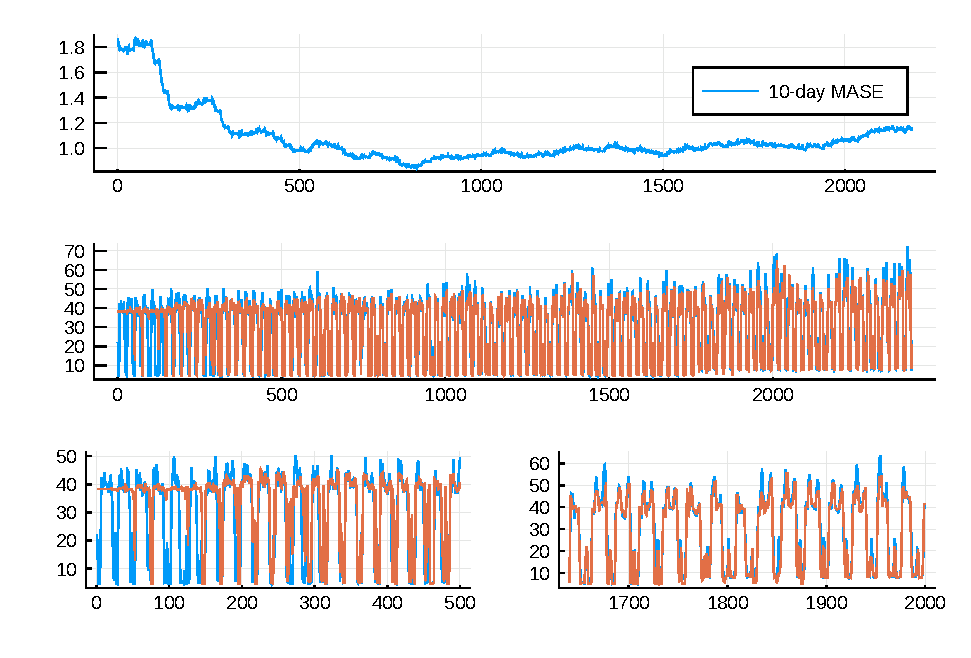
\includegraphics[width=1.05\textwidth,height=.6\textheight]{figures/tm1.eps}
		\caption[μελέτη πρόβλεψης χρονοσειράς με τη χρονική μνήμη]{%
			Μελέτη πρόβλεψης χρονοσειράς με τη χρονική μνήμη.
			Πάνω: εξέλιξη σφάλματος MASE σταθμισμένο σε διάστημα 10 ημερών.
			Μέση: {\color{blue}Χρονοσειρά} και {\color{red} πρόβλεψη}.
			Κάτω: εστίαση του παραπάνω στην αρχική εκμάθηση και στο σημείο αλλαγής της μέσης τιμής.
		}
		\label{fig:tm_tspredict}
	\end{figure}

	\begin{figure}[t]
		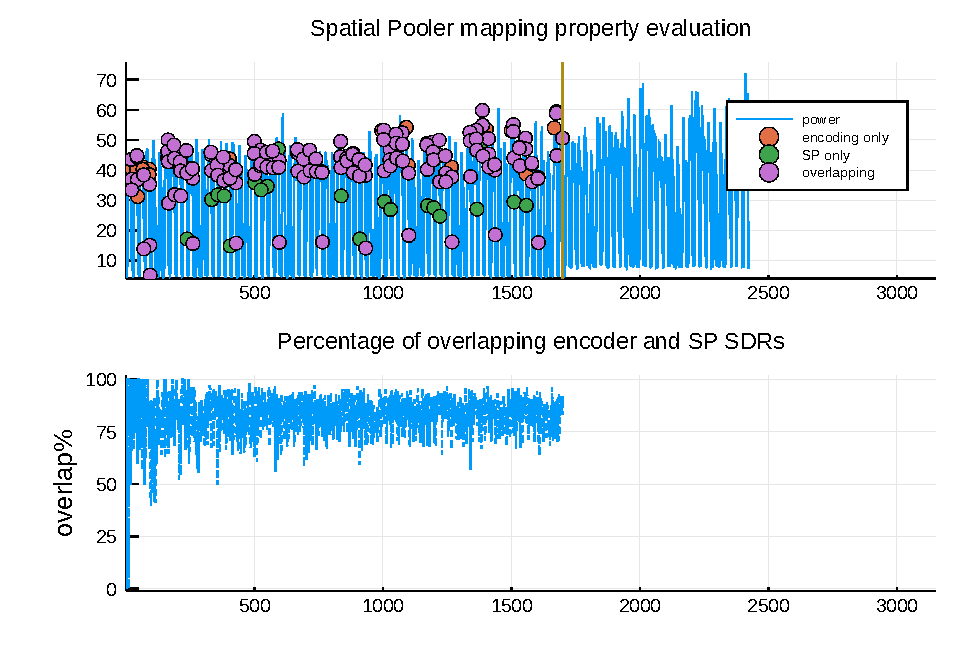
\includegraphics[width=1.1\textwidth]{figures/sp1.eps}
		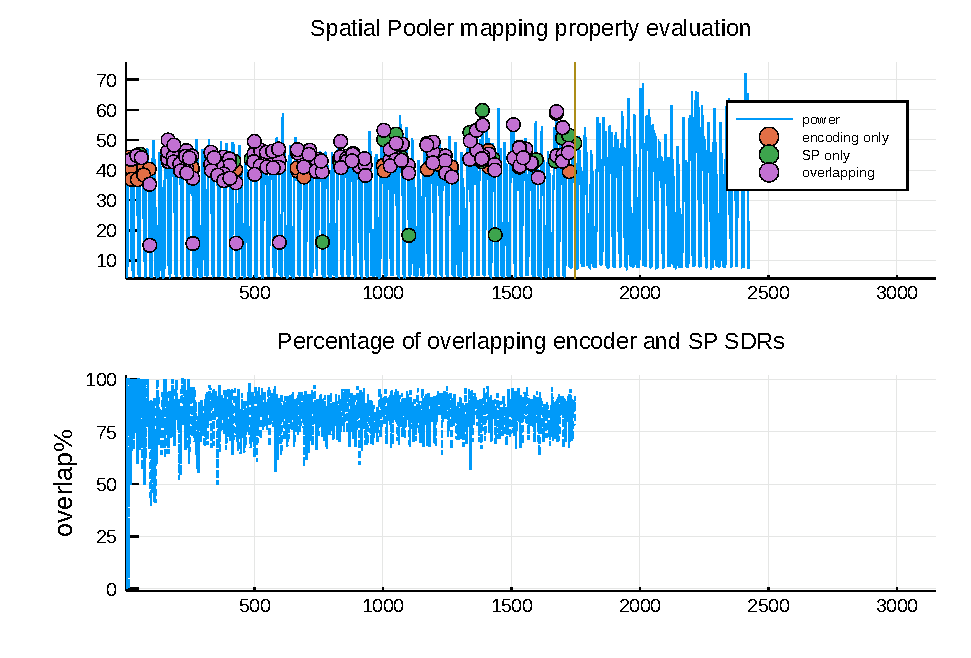
\includegraphics[width=1.1\textwidth]{figures/sp2.eps}
		\caption[]{Μελέτη διατήρησης ομοιότητας του χώρου εισόδου από το χωρικό συγκεντρωτή
		-- αμέσως πριν και μετά την αλλαγή μέσης τιμής της χρονοσειράς}
	\end{figure}
	\begin{figure}[t]\ContinuedFloat
		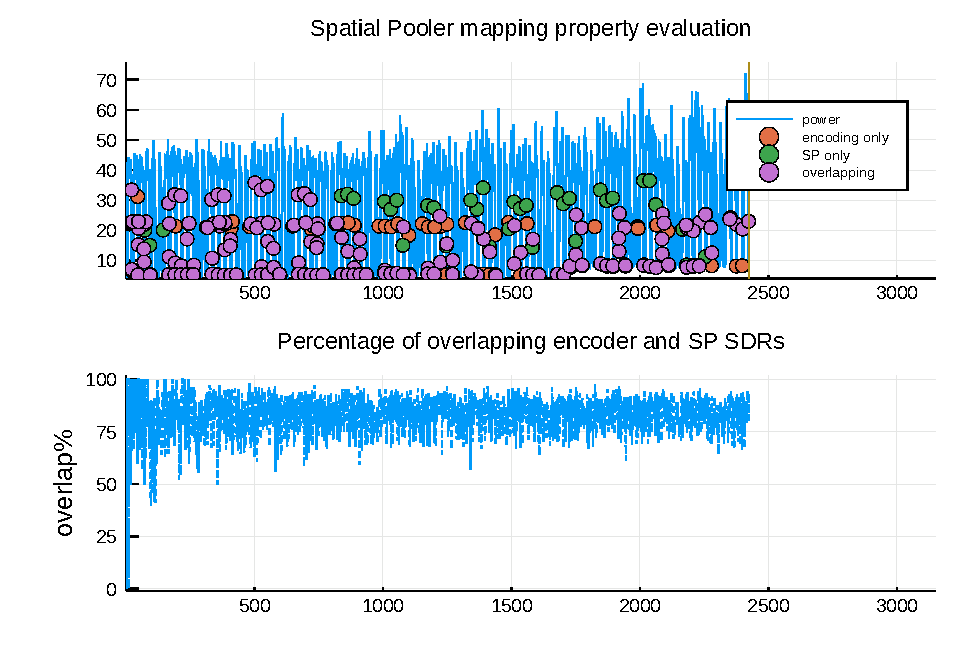
\includegraphics[width=1.1\textwidth]{figures/sp3.eps}

		\captionsetup{singlelinecheck=off}
		\caption[μελέτη διατήρησης ομοιότητας του χώρου εισόδου από το χωρικό συγκεντρωτή]{%
			Μελέτη διατήρησης ομοιότητας από το χώρο εισόδου στο χώρο εξόδου διαμέσου του χωρικού συγκεντρωτή. Αυτή είναι βασική αρχή λειτουργίας του χωρικού συγκεντρωτή
			και η απόδειξη της σχετικής της ισχύος χρησιμεύει τόσο ως τεκμήριο ορθότητας της υλοποίησης,
			όσο και του αλγορίθμου γενικότερα.
			Χρησιμοποιείται η χρονοσειρά που περιγράφεται στο \ref{conc:tspred-dataset}.

			Παρουσιάζονται 3 στιγμιότυπα: αμέσως πριν και αμέσως μετά την αλλαγή της μέσης τιμής της χρονοσειράς και στο τέλος.
			Για κάθε στιγμιότυπο υπάρχουν 2 γραφήματα.

			Στο πάνω φαίνεται η χρονοσειρά και επισημαίνονται τα πιο ταιριαστά ως τώρα SDR με την τρέχουσα στιγμή:
			{\color{red} είσοδοι που δεν ταιριάζουν πολύ με την τωρινή έξοδο},
			{\color{green} έξοδοι που δεν ταιριάζουν πολύ με την τωρινή είσοδο},
			{\color{magenta} είσοδοι και έξοδοι που ταιριάζουν με τις τωρινές}.

			Στο κάτω φαίνεται το ποσοστό των εισόδων/εξόδων που ταιριάζουν. Χρησιμεύει ως μέτρο επίδοσης του χωρικού συγκεντρωτή.

			Φαίνεται πως η αλλαγή της μέσης τιμής έχει αμελητέα επίδραση στην επίδοση του χωρικού συγκεντρωτή.
			Καθώς το πείραμα εξελίσσεται το μέτρο επίδοσης γίνεται πιο εύρωστο, καθώς προκύπτει από περισσότερα SDR.
			Αυτός είναι ο κύριος λόγος που μειώνεται η διακύμανση.
		}
		\label{fig:sp_maintain_similarity}
	\end{figure}


\section{Τι αξίζει να μελετηθεί περαιτέρω;} \label{conc:study-suggestions}

\subsubsection{Αισθητικοκινητική συμπερασματολογία και χρονική συγκέντρωση}

	Οι αλγόριθμοι που παρουσιάστηκαν εδώ αναπτύχθηκαν κυρίως μέχρι τις αρχές του 2017.
	Έκτοτε, η εταιρία Numenta που ηγείται της μελέτης έχει προτείνει πολλές νέες διαστάσεις στη θεωρία HTM.
	Βασική τέτοια είναι η αισθητικοκινητική συμπερασματολογία (sensorimotor inference).
	Βασιζόμενοι στην παρατήρηση ότι η είσοδος σε ένα ενσώματο σύστημα HTM μπορεί να αλλάζει για δύο διαφορετικούς λόγους,
	εξωγενή αλλαγή ή αλλαγή οπτικής γωνίας λόγω κίνησης του ιδίου του σώματος,
	προτείνουν ότι η διαδικασία της πρόβλεψης πρέπει να έχει πρόσβαση σε αντίγραφα των κινητικών εντολών και να τις λαμβάνει υπόψιν \parencite{hawkinsTheoryHowColumns2017}.
	Επίσης εισάγεται η έννοια της θέσης, τόσο του σώματος μέσα στον έξω κόσμο (πχ στο δωμάτιο), όσο και του αισθητήρα ως προς το αντικείμενο.
	Με αυτά τα στοιχεία συντίθεται η δυνατότητα μερικών φλοιικών στηλών που εργάζονται συντονισμένα να δημιουργήσουν μοντέλα φυσικών αντικειμένων και να τα διαχωρίσουν μεταξύ τους.

	Το μοντέλο του φυσικού αντικειμένου συσχετίζεται άμεσα με το μοντέλο μιας ακολουθίας στη χρονική μνήμη.
	Μία προέκταση της θεωρίας HTM που έχει κάποιο θεωρητικό υπόβαθρο αυτή τη στιγμή και χρήζει άμεσης μελέτης είναι
	ο συνδυασμός της χρονικής μνήμης με μία δεύτερη περιοχή που θα μοντελοποιεί ολόκληρες ακολυοθίες εισόδων
	και θα προδιαθέτει τη χρονική μνήμη με ανάδραση από τους κορυφαίους δενδρίτες.
	Ο μηχανισμός αυτός μπορεί να ονομαστεί και «χρονική συγκέντρωση» (temporal pooling).
	Στο παράδειγμα της παρακολούθησης μιας μελωδίας, αν η χρονική μνήμη μαθαίνει να αναπαριστά την τρέχουσα νότα ως προς τις προηγούμενες,
	ο χρονικός συγκεντρωτής μαθαίνει να αναπαριστά μουσικά θέματα.
	Η επιτυχής ενσωμάτωση ενός τέτοιου μηχανισμού αναμένεται να βελτιώσει σημαντικά την ικανότητα πρόβλεψης χρονοσειρών.

	Η χρονική μνήμη όπως παρουσιάστηκε, αν και δεν είναι ευαίσθητη στο θόρυβο του χώρου εισόδου χάρη στο χρονικό συγκεντρωτή,
	είναι πολύ ευαίσθητη στο \textbf{χρονικό θόρυβο}, όπως η ανταλλαγή της σειράς δύο συμβόλων εισόδου.
	Η προδιάθεση από το χρονικό συγκεντρωτή αναμένεται να προσδώσει ευρωστία σε τέτοιας μορφής θορύβου.

	Στο άρθρο \cite{hawkinsTheoryHowColumns2017} παρουσιάζεται μεν ένας μηχανισμός με τον οποίο η HTM μαθαίνει και αναγνωρίζει πολλά ξεχωριστά αντικείμενα,
	αλλά μονάχα με τη βοήθεια εξωγενούς σήμανσης για το πότε τα αντικείμενα αλλάζουν.
	Δεν περιγράφεται δηλαδή μηχανισμός \textbf{συνεχούς μάθησης}, με τον οποίο να μαθαίνονται και τα σύνορα μεταξύ των αντικειμένων.
	Σημαντικό ρόλο σε αυτήν την κατεύθυνση ενδέχεται να διαδραματίσει κάποιος μηχανισμός «έκπληξης», όπως είναι η έξαρση των μικροστηλών της χρονικής μνήμης
	για απροσδόκητες εισόδους.

\subsubsection{Ιεραρχική σύνθεση πολλών περιοχών}

	Αν και το όνομα της θεωρίας ξεκινά με τη λέξη «ιεραρχική», η ιεραρχία δε συμμετείχε σε όσα περιγράφηκαν ως τώρα.
	Η ιεραρχία αρχίζει να συντίθεται στην τρέχουσα θεωρία με ένα πρόσφατο άρθρο \cite{hawkinsFrameworkIntelligenceCortical2019}
	που προτείνει μηχανισμούς συνεργασίας πολλών φλοιικών στηλών.

	Σε πιο πρακτικό επίπεδο, η ιεραρχία φαίνεται να είναι το κλειδί για την πρόβλεψη και αναγνώριση ανωμαλιών σε πολύπλοκα συστήματα
	που εκφράζουν τη συνολική τους κατάσταση με πολλές ταυτόχρονες χρονοσειρές (\textbf{multivariate timeseries prediction}).
	Με μία μόνο περιοχή δεν υπάρχει αποτελεσματικός τρόπος για τη σύνθεση πολλών χρονοσειρών σε ένα χώρο εισόδου.

\subsubsection{Διάφορες ιδέες}

	Οι παραπάνω είναι ίσως οι πιο σημαντικές κατευθύνσεις για περαιτέρω έρευνα, όμως αναγνωρίζονται και πολλά πιο εντοπισμένα ερωτήματα
	ως προς τη συμπεριφορά των αλγορίθμων που περιγράφηκαν.
	\begin{itemize}
		\item Είναι ευσταθείς οι μηχανισμοί εκμάθησης; Πώς επηρεάζονται από τον κβραντισμό των συναπτικών μονιμοτήτων;
		\item Αν δούμε το δίκτυο της χρονικής μνήμης ως γράφο με τοπικούς κανόνες προσαρμογής, είναι ενδιαφέρον να μελετηθεί υπό το πρίσμα του άρθρου \cite{kipouridisConvergenceNetworkSystems2019}
		\item Οι συνάψεις αυτή τη στιγμή είναι δισταθείς (συνδεδεμένες/αποσυνδεδεμένες), αλλά ο μόνος βιολογικός περιορισμός είναι ότι δεν μπορούν να έχουν μεγάλη ακρίβεια.
		Ας μελετηθούν λοιπόν συνάψεις με περισσότερες καταστάσεις, με συναπτικά βάρη 2-3 bit.
	\end{itemize}

	Τέλος, όσον αφορά την παρούσα υλοποίηση, οι ιδιότητες των αλγορίθμων επικυρώθηκαν μόνο αδρομερώς με δύο συνολικούς ελέγχους.
	Η επίσημη υλοποίηση της Numenta έχει μελετηθεί με πολύ περισσότερους ελέγχους, που παρουσιάζονται στα άρθρα τους
	\parencite{cuiHTMSpatialPooler2017,cuiContinuousOnlineSequence2016}.
	Είναι σημαντικό να αναπαραχθούν αυτοί οι έλεγχοι, ώστε να τεκμηριωθούν και οι υπόλοιπες ιδιότητες του χωρικού συγκεντρωτή και της χρονικής μνήμης.


\section{Συμπέρασμα}

	Στην εργασία αυτή παρουσιάστηκε η θεωρία HTM, μαζί με το βιολογικό υπόβαθρο που προσπαθεί να ερμηνεύσει,
	και μια υλοποίηση των κεντρικών της αλγορίθμων σε νέα γλώσσα μαθηματικού προγραμματισμού, τη Julia.

	Οι αλγόριθμοι είναι περίπλοκοι και σχετικά πολύπλοκοι, όχι ως προς την υπολογιστική τους πολυπλοκότητα,
	αλλά ως προς τη δυσκολία στην περιγραφή των πολλών εννοιών που περιλαμβάνουν.
	Η υλοποίηση του χωρικού συγκεντρωτή σε 120 γραμμές κώδικα και της χρονικής μνήμης σε 222,
	σε αντιδιαστολή με την πρότυπη υλοποίηση των αλγορίθμων σε 700 και 750 γραμμές αντίστοιχα,
	θεωρείται ότι μπορεί να αποτελέσει μια αποτελεσματική περίληψη των αλγορίθμων και ταυτόχρονα σαφή τους διατύπωση.
	Η επιτυχία του κεντρικού αυτού στόχου της εργασίας, όμως, θα μπορέσει να αξιολογηθεί μόνο στο μέλλον, με το κατά πόσον πράγματι θα αποτελέσει βάση για περαιτέρω μελέτη.

	Η υλοποίηση απαιτούσε τη βαθιά κατανόηση της Julia.
	Χρησιμοποιήθηκαν και παρουσιάστηκαν προχωρημένες δυνατότητες της γλώσσας όπως μοτίβα σχεδιασμού με παραμετρικές μεθόδους και πολλαπλή αποστολή,
	χαμηλού επιπέδου χειρισμοί με αραιούς πίνακες, μακροεντολές, μετρήσεις απόδοσης (benchmarking) και άλλα.
	Οδήγησε επίσης στη συνεισφορά στην πηγή της επίλυσης μερικών προβλημάτων, στο πλαίσιο της ανάπτυξης ενός παγκόσμιου εύρους ανοιχτού λογισμικού.

	Οι αλγόριθμοι δοκιμάστηκαν με βασικούς ελέγχους και η λειτουργικότητά τους επιδείχτηκε.
	Παρατηρήθηκε βέβαια ότι, στην παρούσα μορφή, δεν είναι ιδιαίτερα αποτελεσματικοί στο πρόβλημα της πρόβλεψης,
	και ότι χρειάζονται περισσότερη μελέτη και πειραματισμό με ήδη προταθείσες θεωρητικές βελτιώσεις.

	Εν τέλει, αναφέρθηκαν πιθανές προεκτάσεις για περαιτέρω μελέτη, καταδεικνύοντας και πώς ενδέχεται να βελτιωθεί η απόδοση των αλγορίθμων
	και πώς αυτή η εργασία μπορεί να φανεί χρήσιμη.
